\documentclass[a4paper]{usiinfbachelorproject}

\captionsetup{labelfont={bf}}
%%%%%%%%%%%%%%%%%%%%%%%%%%%% PACKAGES %%%%%%%%%%%%%%%%%%%%%%%%%%%%%
\usepackage{float}
\usepackage{amsmath}
\usepackage{todonotes}
% \usepackage[disable]{todonotes} % Disables all TODOs
\usepackage{tikz}
\usetikzlibrary{arrows.meta, positioning}

%%% Main Body %%%

\author{Davide Frova}

\title{\textbf{Exploring the Learning by Teaching with Social Robots}}
\subtitle{Enabling Exploratory Studies on Learning by Teaching with Social Robots through Wizard-of-Oz Control}
\versiondate{\today}

\begin{committee}
%With more than 1 advisor an error is raised...: only 1 advisor is allowed!
\advisor[Istituto Dalle Molle di Studi sull\'Intelligenza Artificiale, IDSIA, Switzerland]{ }{Monica}{Landoni}
%You can comment out  these lines if you don't have any assistant
\coadvisor[Istituto Dalle Molle di Studi sull\'Intelligenza Artificiale, IDSIA, Switzerland]{ }{Antonio}{Paolillo}

\end{committee}

\abstract { Abstract goes here ...
You may include up to six keywords or phrases. Keywords should be separated with semicolons. 
\\
\textbf{Keywords}:

}
\begin{document}
\maketitle
\tableofcontents\newpage
%\listoffigures\newpage

\section{\textbf{Introduction}}
\todo[inline]{Will rewrite when working on the abstract, need to write about already existing tools. Currently, this is a mixup of the abstract and the introduction.}

Social robots are increasingly finding their way into learning environments, where their role as collaborators, tutors, or learning companions is being actively explored. In particular, the paradigm of \textit{Learning by Teaching} (LbT) offers a promising framework in which children can reinforce their understanding and social-emotional skills by teaching a robot. This approach has the potential to enhance engagement, improve soft skills, and support inclusive education.

This bachelor project is part of the broader TESORO initiative, for which an SNSF funding application has been submitted and is currently awaiting approval. My contribution focuses on a practical implementation: the design and development of a web-based dashboard that enables a Wizard-of-Oz control of a social robot during an exploratory experiment involving turn-taking with children.

The experiment consists of a Lego-building task performed by two children taking turns. The robot, remotely controlled via the dashboard, intervenes when turn-taking violations occur, aiming to regulate the interaction and reinforce collaborative behavior.

This report presents the background of the project, the research and implementation goals, the technical architecture of the system, and the planned experimental study.
The developed dashboard serves as a starting point for preliminary studies and lays the groundwork for later stages of the TESORO project where the robot will learn these regulatory behaviors from various operators, including researchers, teachers, or even the children themselves. Additionally, it could also serve other projects that are based on Human-Robot Interaction (HRI) since it will be developed in a way that is re-usable for different scenarios.

\subsection{\textbf{Report structure}}
The rest of the report is organized as follows: Section~\ref{sec:background} presents the related work and theoretical framework; Section~\ref{sec:design} outlines the experiment scenario and research goals; Section~\ref{sec:system} describes the dashboard's architecture and implementation; Section~\ref{sec:evaluation} discusses the system's current status and outlines the upcoming evaluation; and Section~\ref{sec:conclusions} concludes with future directions.


\section{\textbf{State of the art}}\label{sec:background}
\todo[inline]{Here we will summarize the main findings, carefully explain the differences with our work and could have a small "background information" section.}
\textit{
    Explain all acronyms and abbreviations. For example, the first time an acronym is used, write it out in full and place the acronym in
    parentheses. When using the Graphical User Interface (GUI) version, the use may...
}


\section{\textbf{Experiment Design and Goals}}\label{sec:design}

The experiment designed for this project aims to explore how a social robot can support children's learning through turn-taking regulation. The overall investigation is structured into three progressive stages:

\begin{itemize}
    \item \textbf{Step 1: Robot as Regulator} - Two children collaboratively build a Lego tower by taking turns. The robot observes and intervenes in case of turn violations, using multimodal cues such as LED lights, vocalizations, and gestures.
    \item \textbf{Step 2: Child as Regulator} - A child is tasked with regulating the interactions between the robot and another child that will perform a similar task to Step 1. This step exploits the LbT paradigm, where the regulator learns how to collaborate and keep turns.
    \item \textbf{Step 3: Robot Learns How and When to Intervene} - The robot applies the learned behavior during interactions with children in Step 1 and Step 2.
\end{itemize}

This report provides the foundational knowledge for implementing later stages of autonomous learning. The robot's interventions are controlled via a Wizard-of-Oz setup, and the primary goal is to assess the feasibility and effectiveness of such interventions in developing children's soft skills.


\section{\textbf{System Design and Implementation}}\label{sec:system}

\subsection{\textbf{System Architecture}}
\subsection*{\textbf{Overview}}
The system architecture was designed to enable an operator to control a social robot in a Wizard-of-Oz fashion during experiments with children.
The main components include a web-based dashboard for real-time control~\cite{frovaaa2025hogwarts}, a communication layer based on ROS2 (Robot Operating System 2)~\cite{ros2, frovaaa2025robomaster, frovaaa2025robomasterhri}, and the RoboMaster EP robot~\cite{djirobomasterep}.
The dashboard provides intuitive controls for triggering robot interventions and monitoring status, while the ROS2 integration ensures reliable communication and execution of commands.
This architecture prioritizes usability, low latency, and safety, supporting the experimental requirements for responsive and effective interactions.
The system was designed to facilitate iterative development and easy modifications, supporting a co-design approach as outlined in the TESORO project proposal~\cite{landoni2025tesoro}.
This flexibility enables rapid adaptation of the dashboard based on feedback from stakeholders and participants during the study.

\subsection{\textbf{Component Description}}
\subsubsection*{\textbf{Dashboard}}
The dashboard is a web-based interface developed using Next.js, with the user interface built on Material UI (MUI) components for a modern and consistent look.
It allows the operator to monitor the robot's status and trigger interventions in real time. Communication with the robot is achieved via \texttt{roslibjs}~\cite{roslibjs}, which enables the dashboard to send and receive ROS messages over the network.

\subsubsection*{\textbf{Middleware Server}}
Due to a known limitation in \texttt{roslibjs} when interacting with ROS2 action servers, a minimal middleware server was implemented within the dashboard system.
This server is built with Express and uses \texttt{rclnodejs}~\cite{rclnodejs} to interface directly with ROS2, acting as a bridge between the dashboard and ROS2 action servers.
This ensures reliable execution of complex robot actions and exposes additional functionalities to the web interface.

\subsubsection*{\textbf{ROS Communication Layer}}
The communication layer is based on ROS2 and uses \texttt{rosbridge\_server}~\cite{rosbridge} running on the Ubuntu machine that controls the robot ROS2 drivers.
This layer handles the communication between the dashboard and the robot, allowing for real-time updates and command execution.

\subsubsection*{\textbf{Robot Control and Action Servers}}
The Ubuntu machine runs several ROS2 nodes and action servers, including:
\begin{itemize}
    \item \texttt{robomaster\_ros}~\cite{frovaaa2025robomaster}: ROS2 drivers for the RoboMaster EP robot, providing low-level control and sensor access.
    \item \texttt{robomaster\_hri}~\cite{frovaaa2025robomasterhri}: Custom packages for high-level robot control and human-robot interaction.
    \item Security and safety action servers: Allow the operator to immediately halt robot actions or trigger safety protocols as needed.
\end{itemize}

\subsubsection*{\textbf{RoboMaster EP Robot}}
The RoboMaster EP robot~\cite{djirobomasterep} is the physical platform used for the experiment.
It connects to the Ubuntu machine via its dedicated access point, ensuring a stable and isolated communication channel.
The robot executes commands received from the ROS2 action servers and ROS2 nodes, and provides feedback to the dashboard.


\subsubsection*{\textbf{Network and Deployment}}
All components are deployed on a local network to ensure low latency and reliability.
The dashboard can be accessed from any device on the network, while the Ubuntu machine acts as the central hub for ROS2 communication and robot control.
Since the RoboMaster EP robot connects wirelessly and provides odometry data, the system is not restricted to a laboratory setting.
This flexibility allows experiments and interactions with children to take place in more neutral or familiar environments, which can be beneficial for naturalistic studies and participant comfort.

\subsection{\textbf{Safety Considerations}}
Ensuring the safety of participants and equipment was a primary concern throughout the system design.
To address this, a dedicated ROS2 node was developed to act as an emergency stop mechanism.
This node can immediately halt all ongoing robot actions and stop the RoboMaster EP's motors.

A prominent "Emergency Stop" button is integrated into the dashboard interface, allowing the operator to trigger this safety mechanism at any time during an experiment.
When activated, the command is sent via the ROS2 communication layer to the safety node running on the Ubuntu machine, ensuring a rapid response.
This feature is essential for experiments involving children, as it provides the operator with immediate control to prevent unintended or unsafe robot behavior.
The system was tested to ensure that the emergency stop reliably overrides all other commands and brings the robot to a safe state.

\subsection{\textbf{System Architecture Diagram}}

\begin{figure}[H]
    \centering
    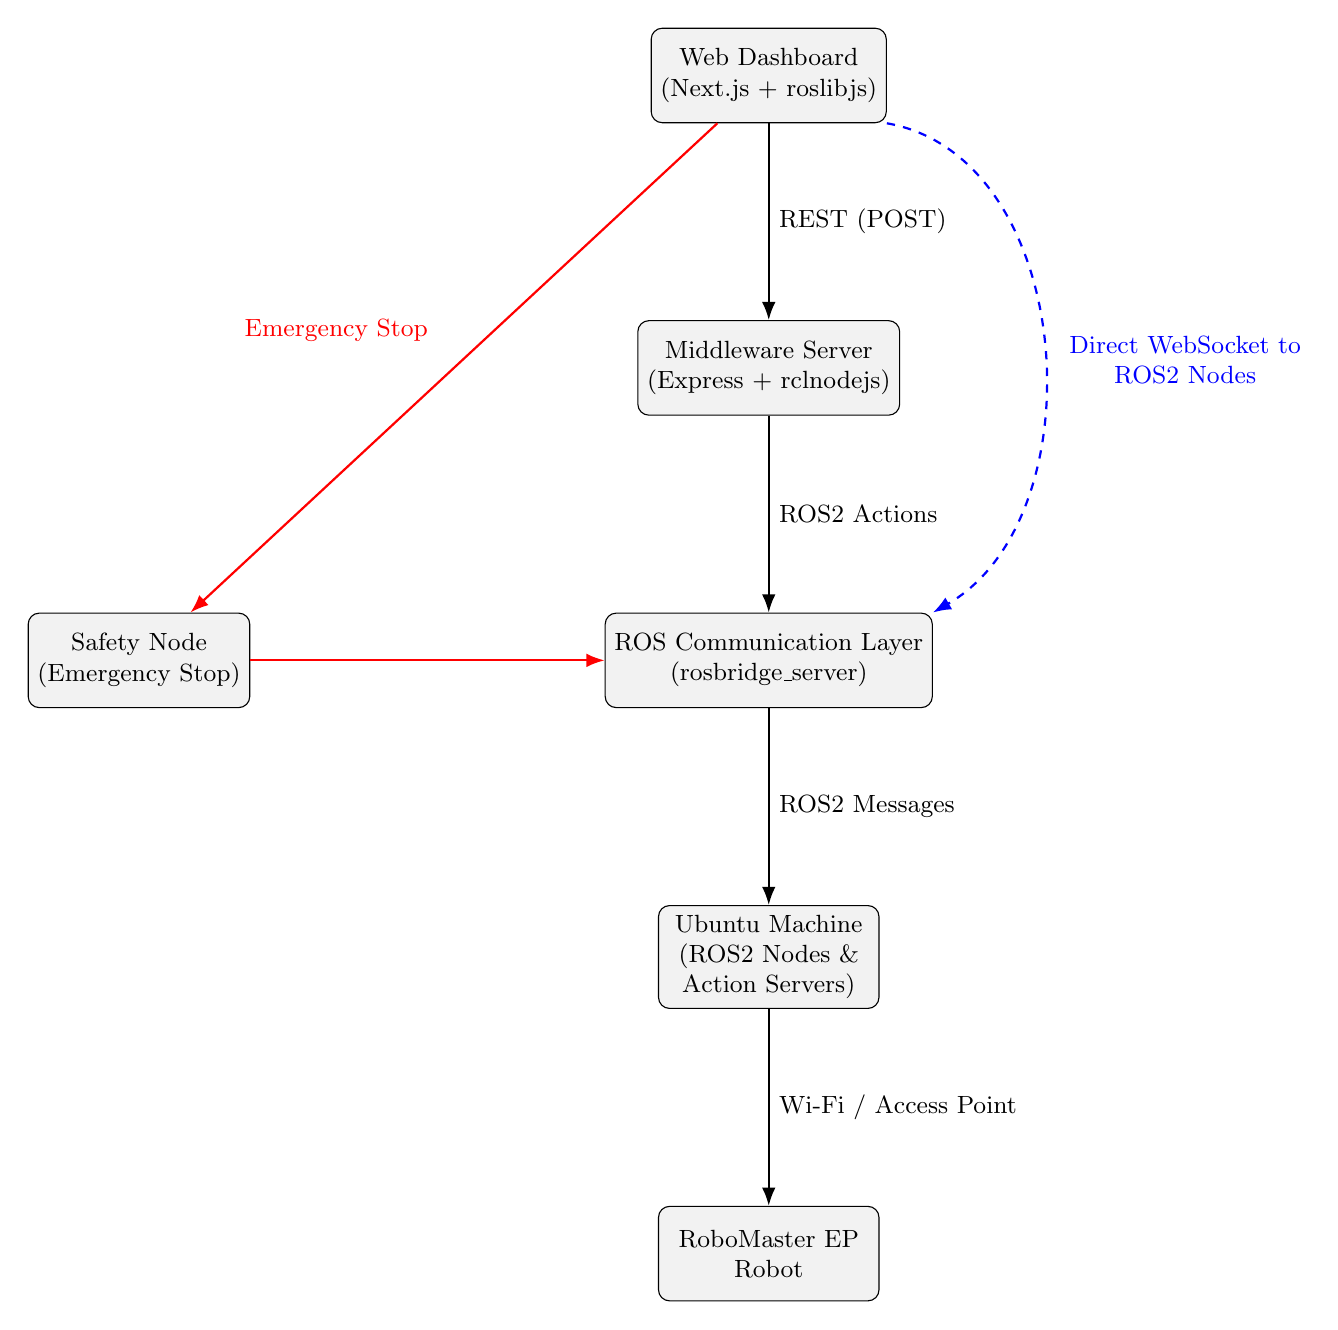
\begin{tikzpicture}[
            node distance=2.5cm and 2.5cm,
            every node/.style={font=\small, align=center},
            box/.style={draw, rounded corners, minimum width=2.8cm, minimum height=1.2cm, fill=gray!10},
            arrow/.style={-Latex, thick}
        ]

        % Nodes
        \node[box] (dashboard) {Web Dashboard\\ (Next.js + roslibjs)};
        \node[box, below=of dashboard] (middleware) {Middleware Server\\ (Express + rclnodejs)};
        \node[box, below=of middleware] (rosbridge) {ROS Communication Layer\\ (rosbridge\_server)};
        \node[box, below=of rosbridge] (ubuntu) {Ubuntu Machine\\ (ROS2 Nodes \&\\ Action Servers)};
        \node[box, below=of ubuntu] (robot) {RoboMaster EP\\ Robot};

        % Connections
        \draw[arrow] (dashboard) -- node[right] {REST (POST)} (middleware);
        \draw[arrow] (middleware) -- node[right] {ROS2 Actions} (rosbridge);
        \draw[arrow] (rosbridge) -- node[right] {ROS2 Messages} (ubuntu);
        \draw[arrow] (ubuntu) -- node[right] {Wi-Fi / Access Point} (robot);

        % Direct connection from dashboard to ubuntu (ROS2 Nodes)
        \draw[arrow, dashed, blue] (dashboard.south east) to[out=-10,in=30] node[right, xshift=2mm, yshift=-2mm, text=blue] {Direct WebSocket to\\ROS2 Nodes} (rosbridge.north east);

        % Emergency stop
        \node[box, left=4.5cm of rosbridge] (safety) {Safety Node\\ (Emergency Stop)};
        \draw[arrow, thick, red] (dashboard) -- node[above left, xshift=-2mm, yshift=2mm, text=red] {Emergency Stop} (safety);
        \draw[arrow, thick, red] (safety) -- (rosbridge);

    \end{tikzpicture}
    \caption{System architecture for Wizard-of-Oz control of the RoboMaster EP robot. The dashboard communicates with the middleware server via REST (POST request), and can also communicate directly with the ROS2 nodes using WebSocket (roslibjs).}
    \label{fig:system-architecture}
\end{figure}

\subsection{\textbf{Dashboard Interface}}
\todo[inline]{
    Here we will describe the dashboard interface, including the main features and functionalities.
    We will also include screenshots of the dashboard to illustrate its design and layout.
}

\section{\textbf{Evaluation and Current Status}}\label{sec:evaluation}

The current implementation of the dashboard is functional and has been tested with the DJI RoboMaster EP robot. It successfully supports all necessary actions for the experiment.

A pilot study is planned where the dashboard will be used to conduct an initial session of the Lego tower-building task with two children. The operator will use the dashboard to regulate turn-taking behavior. Key observations will include:
\begin{itemize}
    \item Effectiveness of the robot's interventions.
    \item Children's responsiveness to the robot.
    \item Ease of use of the dashboard by the operator.
\end{itemize}

These observations will guide the refinement of both the experiment protocol and the dashboard interface.

\subsection{\textbf{Walkthrough with Experts}}
\subsection*{\textbf{Setup and procedure}}
-
\subsection*{\textbf{Key observations}}
-
\subsection*{\textbf{Design implications}}
-

\subsection{\textbf{Walkthrough with High School Students}}
\subsection*{\textbf{Setup and procedure}}
-
\subsection*{\textbf{Key observations}}
-
\subsection*{\textbf{Design implications}}
-

\subsection{\textbf{Pilot with Children}}
\subsection*{\textbf{Setup and procedure}}
-
\subsection*{\textbf{Key observations}}
-
\subsection*{\textbf{Design implications}}
-

\subsection{\textbf{Summary of Key Iterative Changes}}


\todo[inline]{
    Here we will summarize the key changes made to the dashboard based on the feedback received from the walkthroughs and pilot study.
    This section will highlight the iterative design process and how user feedback informed the development of the system.
}


\newpage

\section{\textbf{Conclusions}}\label{sec:conclusions}
This project presents the design and implementation of a web-based dashboard to enable Wizard-of-Oz control of a social robot used in a Learning by Teaching experiment with children. The system is part of the larger TESORO initiative and lays the groundwork for studying how social robots can assist in learning soft skills like turn-taking.

\subsection{\textbf{Future Work}}
\todo[inline]{
    Here we will write about future work like the ones mentioned in the TESORO project proposal like :
    Long-term goal: enabling real-time learning from the child's regulatory actions and shifting toward semi-autonomous robot behavior.
}


%%%%% BIBLIOGRAPHY %%%%%
\bibliographystyle{abbrv}
\bibliography{references}

\end{document}
